\section{工程制图}

根据最终设计结果，绘制凯尔纳目镜各光学元件的工程制图，包括各透镜与镜组的外形尺寸、曲率半径、中心厚度、边缘厚度、口径、材料标注等，以指导实际加工生产。

\begin{figure}[H]
  \centering
  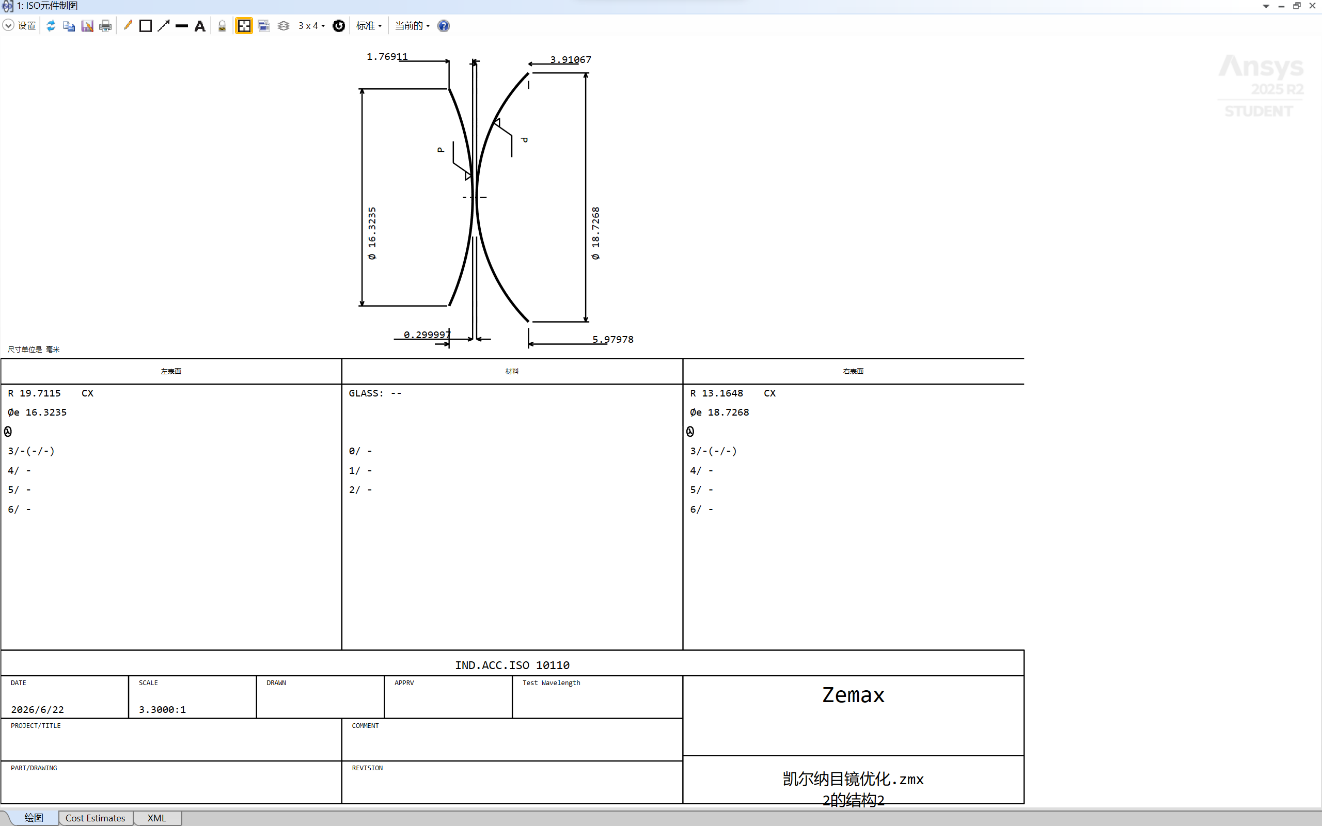
\includegraphics[width=0.95\textwidth]{chapters/chapter10/figures/image18.png}
  \caption{场镜（平凸透镜）工程制图}
  \label{fig:chapter10-field-lens-drawing}
\end{figure}

\begin{figure}[H]
  \centering
  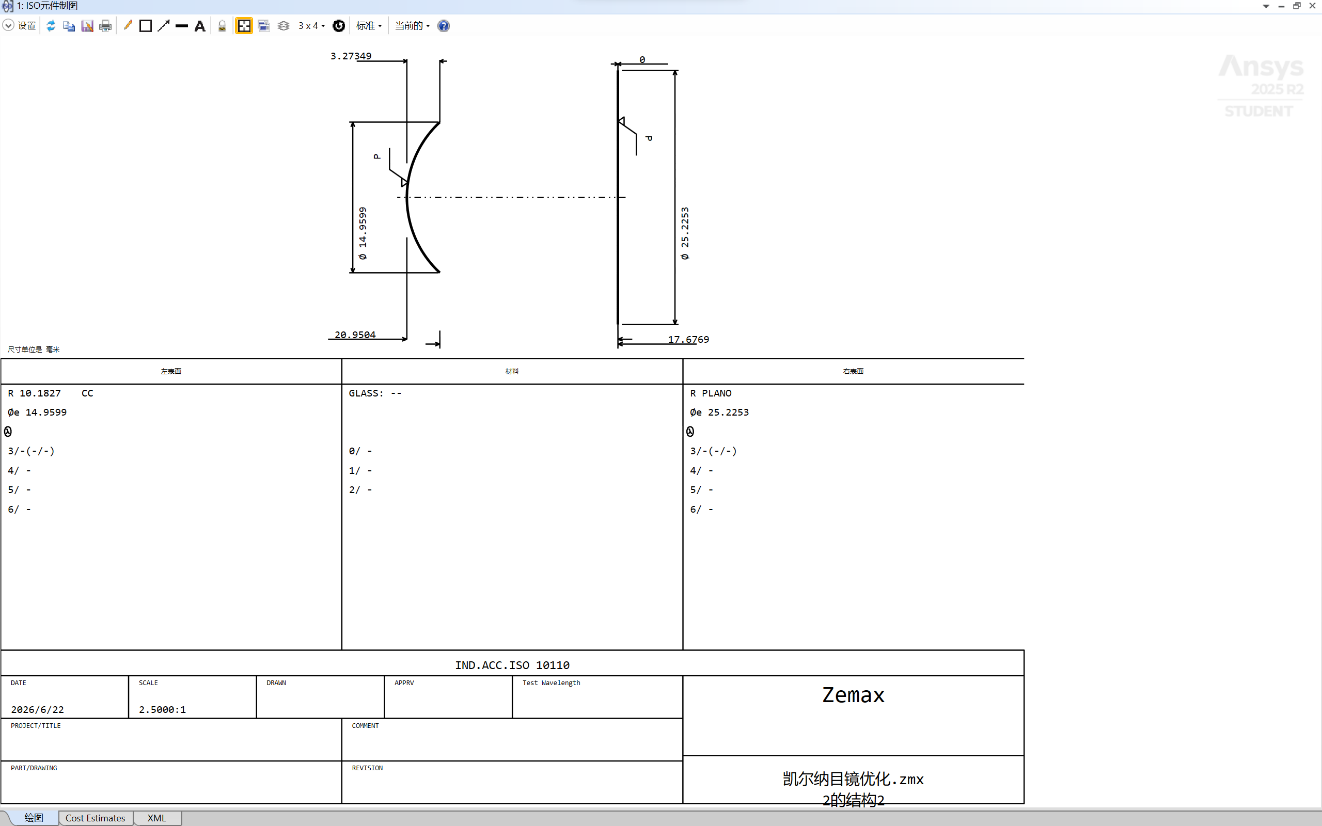
\includegraphics[width=0.95\textwidth]{chapters/chapter10/figures/image19.png}
  \caption{消色差镜组工程制图}
  \label{fig:chapter10-achromatic-doublet-drawing}
\end{figure}

\begin{figure}[H]
  \centering
  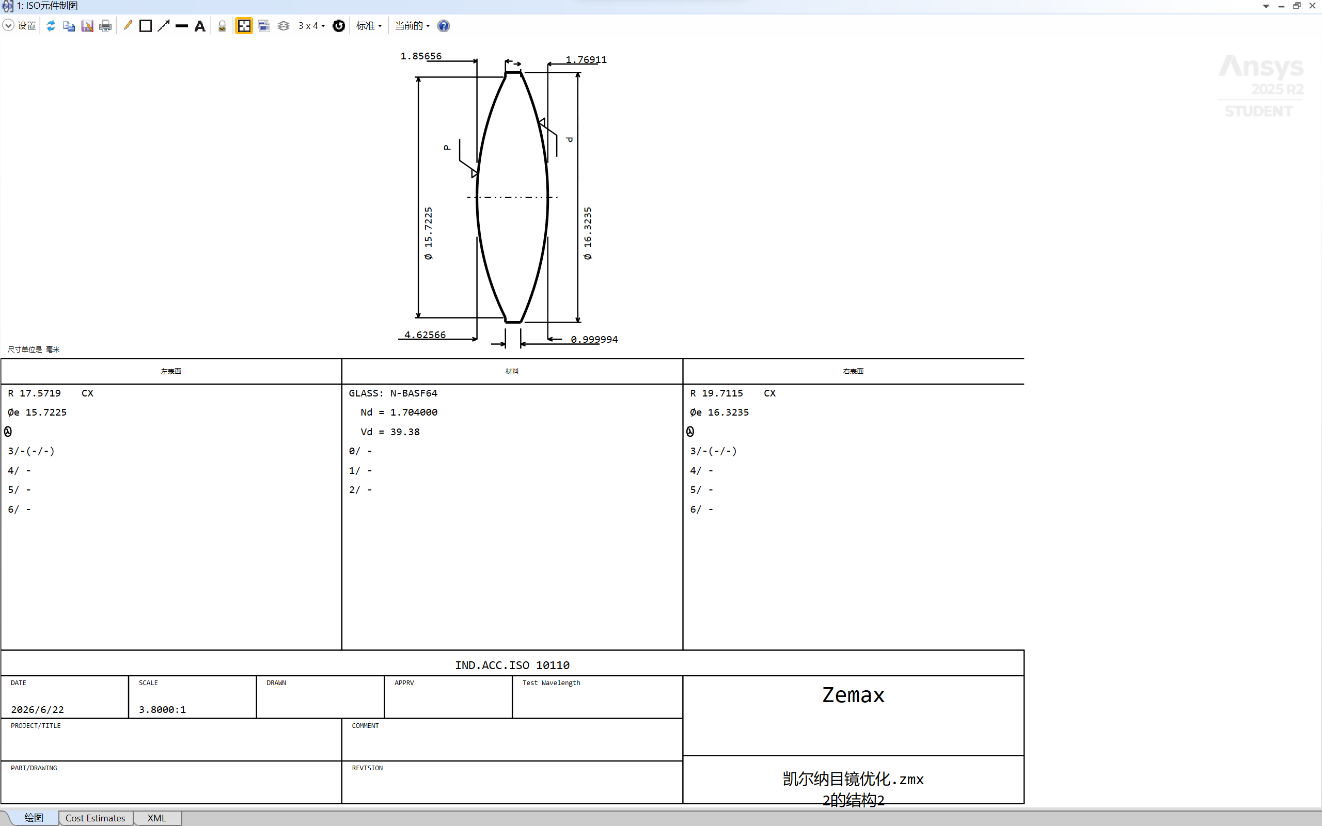
\includegraphics[width=0.95\textwidth]{chapters/chapter10/figures/image20.png}
  \caption{目镜组装配图（含尺寸链标注）}
  \label{fig:chapter10-eyepiece-assembly-drawing}
\end{figure}

\begin{figure}[H]
  \centering
  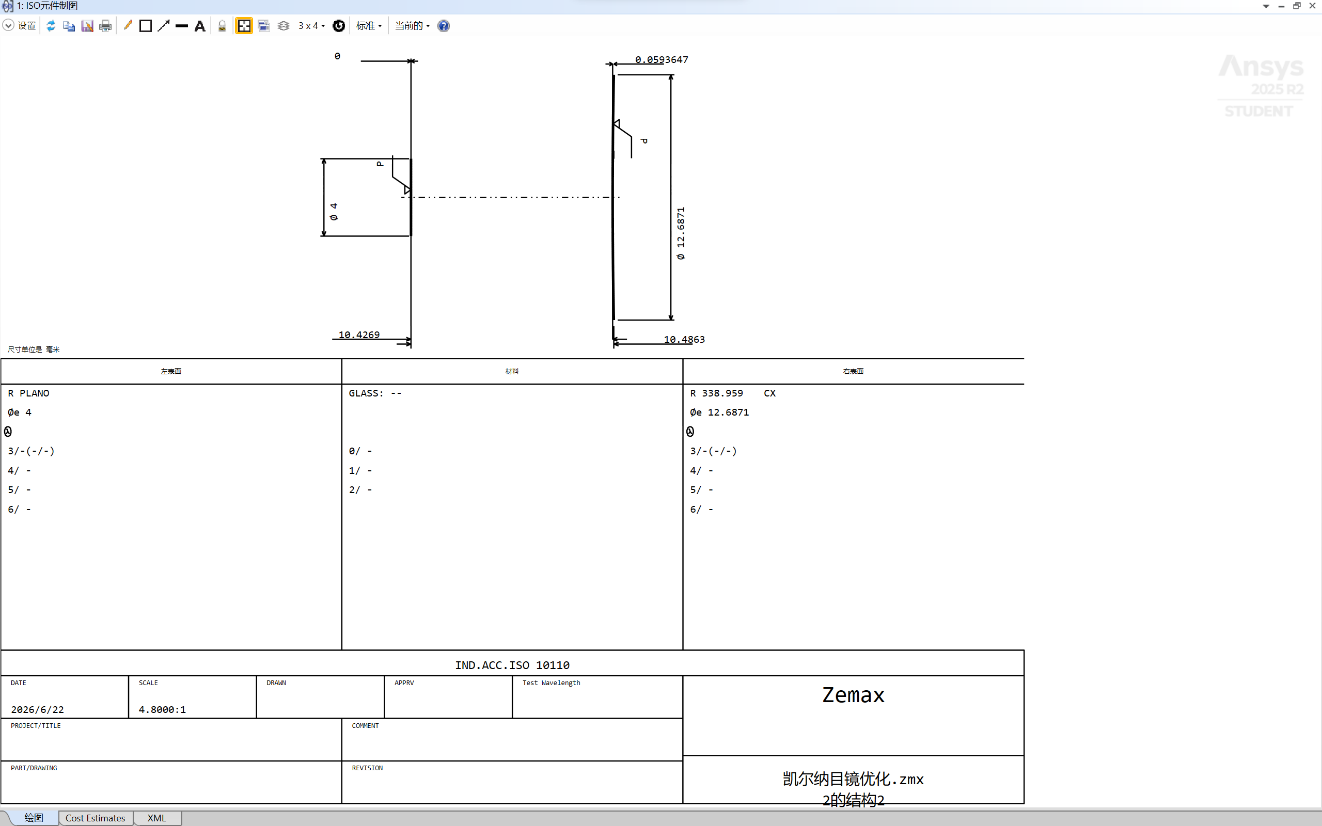
\includegraphics[width=0.95\textwidth]{chapters/chapter10/figures/image21.png}
  \caption{目镜组装配工程制图（一）}
  \label{fig:chapter10-assembly-detail-1}
\end{figure}

\begin{figure}[H]
  \centering
  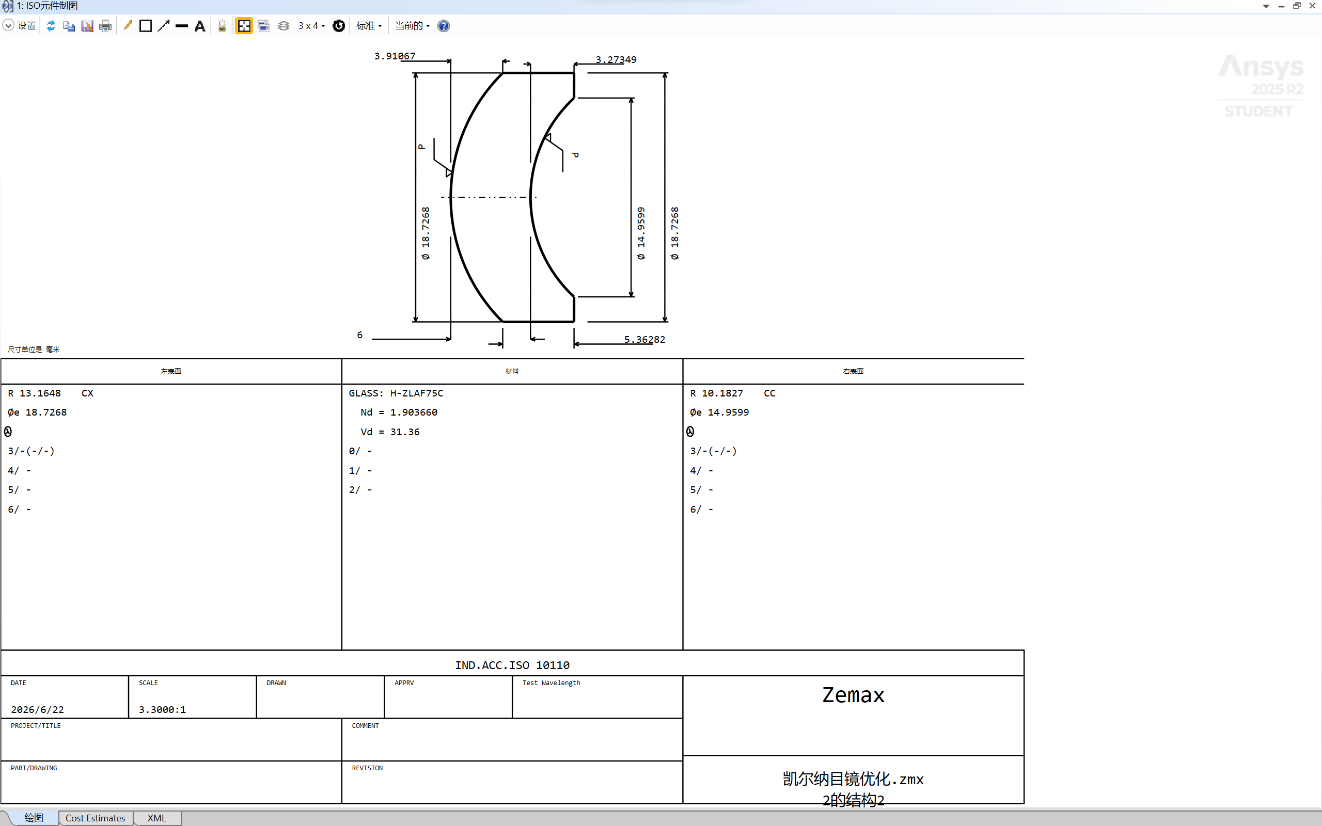
\includegraphics[width=0.95\textwidth]{chapters/chapter10/figures/image22.png}
  \caption{目镜组装配工程制图（二）}
  \label{fig:chapter10-assembly-detail-2}
\end{figure}

\begin{figure}[H]
  \centering
  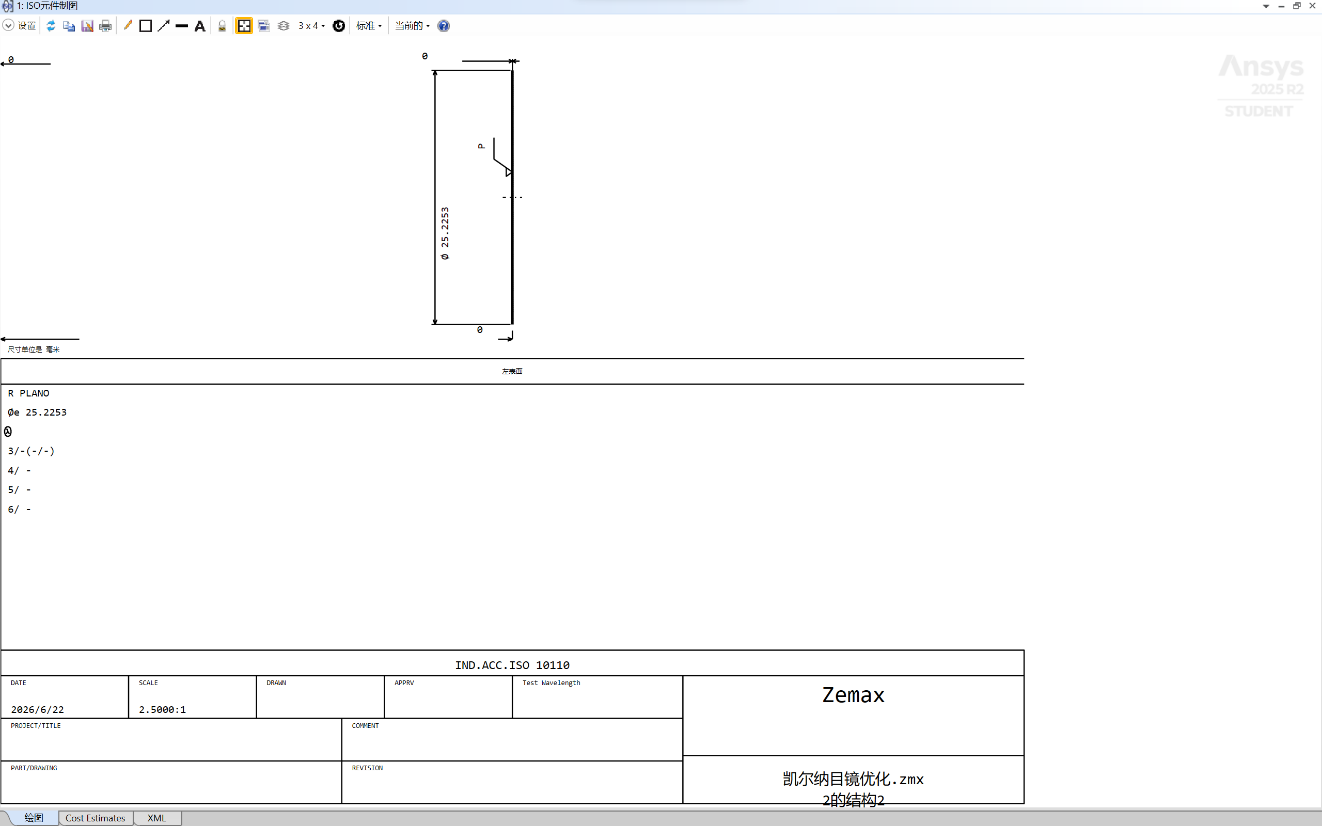
\includegraphics[width=0.95\textwidth]{chapters/chapter10/figures/image23.png}
  \caption{目镜组装配工程制图（三）}
  \label{fig:chapter10-assembly-detail-3}
\end{figure}

\begin{figure}[H]
  \centering
  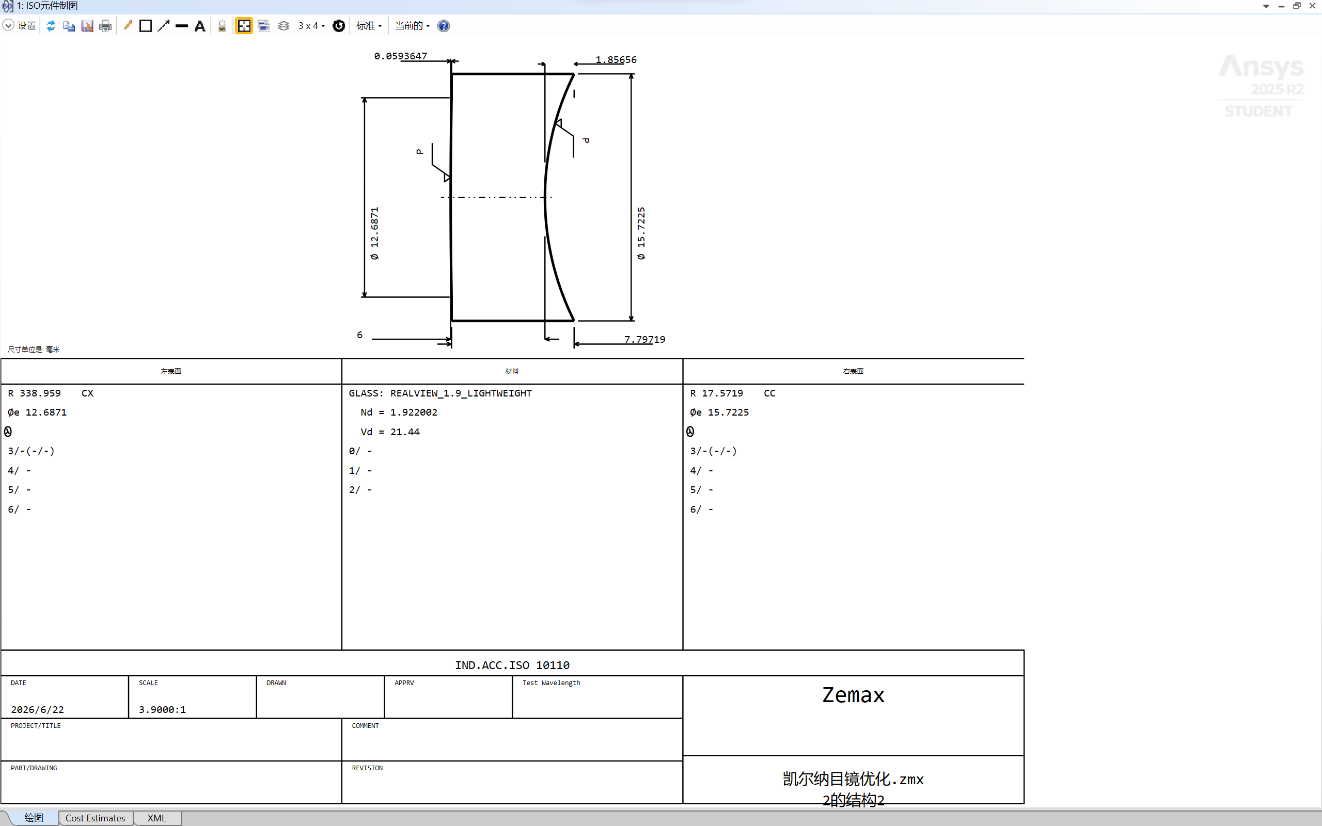
\includegraphics[width=0.95\textwidth]{chapters/chapter10/figures/image24.png}
  \caption{凯尔纳目镜整体装配示意图}
  \label{fig:chapter10-kellner-eyepiece-assembly}
\end{figure}
